\documentclass{beamer}

\usepackage{beamerthemesplit}
\usetheme{Boadilla}
\usepackage[utf8]{inputenc}
\usepackage[russian]{babel}
\usepackage{listings}
\usepackage{color}
\usepackage{hyperref}
\usepackage{tikz}

\usetikzlibrary{arrows,shapes,positioning}


\title{Вычисления в NLO QCD и EW приближении с помощью mcsanc-v1.0}
\author[А.~Сапронов]{Андрей Сапронов}
\institute[ЛЯП ОИЯИ]{ЛЯП ОИЯИ}
\date{24.02.2014}

\begin{document}

\titlepage

\frame{
  \frametitle{Достижения LHC}
  \begin{enumerate}
    \item LHC {\color{red!80} RUN-I}
    \begin{itemize}
      \item Стабильные протон-протонные пучки с 2009 по 2012гг с постепенным повышением {\color{green}энергии от 450GeV до 4TeV}
      \item Основные периоды набора данных 2011 и 2012: \\
        {\color{blue!80} -- \(5{\mathrm{fb}}^{-1} \,@ \,7\mathrm{TeV}\)}\\
        {\color{blue!80} -- \(20{\mathrm{fb}}^{-1} \,@ \,8\mathrm{TeV}\)}
      \item Открыт {\color{red!80} бозон Хиггса} экспериментами  ATLAS и CMS
    \end{itemize}
    \item Результативность детектора {\color{blue!80}ATLAS}:
    \begin{itemize}
      \item Зарегистрировано \(\sim 25{\mathrm{fb}}^{-1}\) интегральной светимости
      \item Загрузка детектора по времени составила \(>99\%\)
      \item Эффективность отбора данных \(\sim 93.5\%\)
    \end{itemize}
  \end{enumerate}
  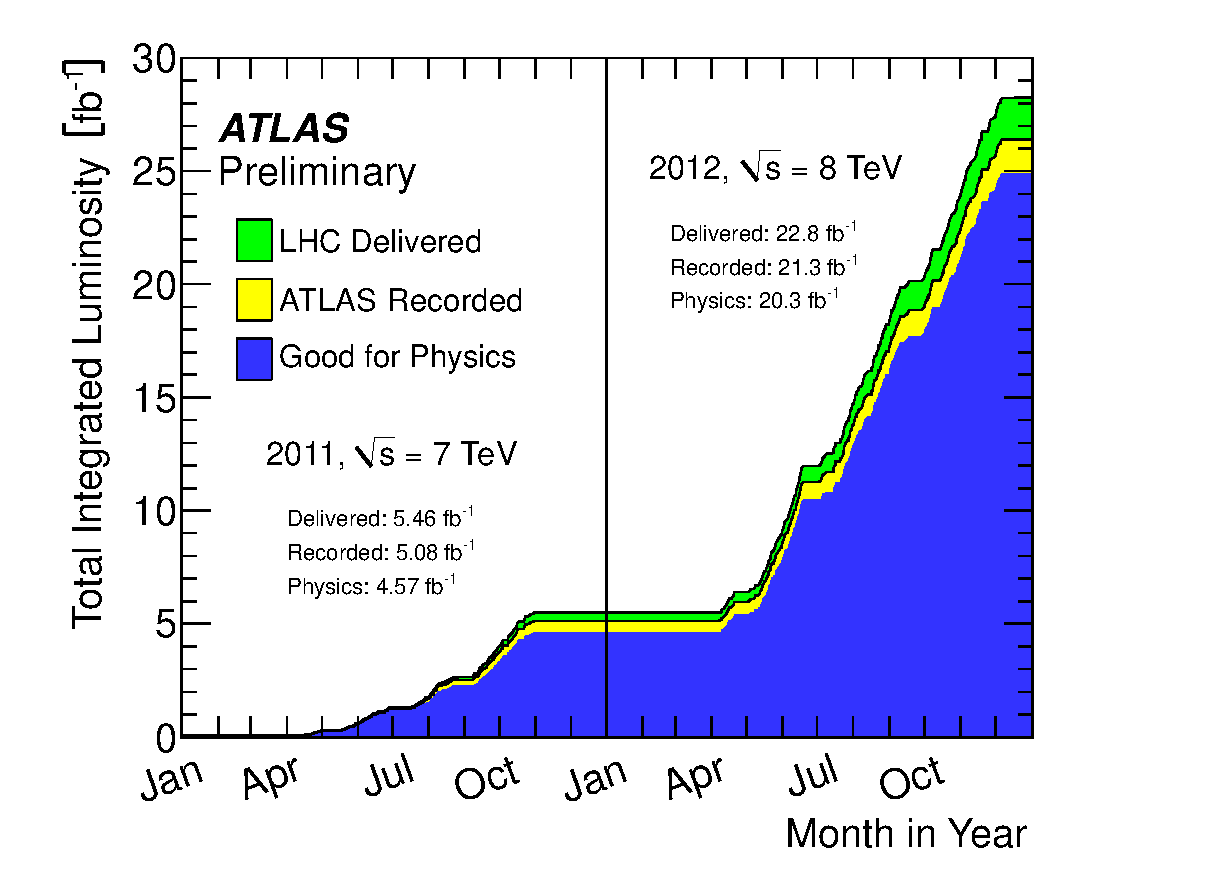
\includegraphics[width=0.4\textwidth]{figs/intlumivstime2011-2012DQ}
  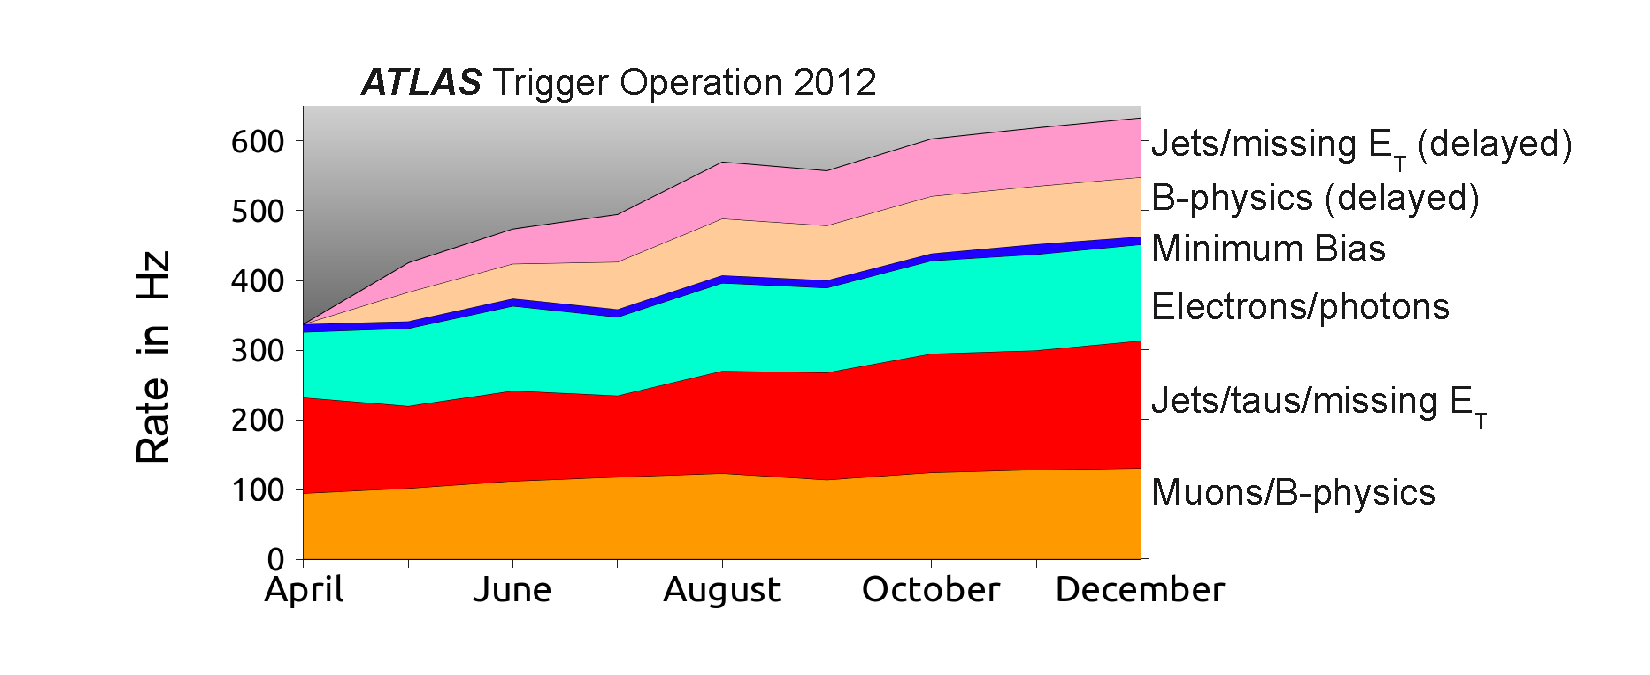
\includegraphics[width=0.6\textwidth,height=3.5cm, clip=true, trim=1cm 0 0 0]{figs/StreamRates2012.pdf}
}

\begin{frame}
  \frametitle{Пример анализа в ATLAS.}
  {\footnotesize
  
  \tikzstyle{bbox} = [draw, thin, fill=blue!20]
  \tikzstyle{gbox} = [draw, thin, fill=green!20]
  
  \begin{figure}
  \begin{tikzpicture}[node distance=3cm, auto,>=latex', thick]
      % We need to set at bounding box first. Otherwise the diagram
      % will change position for each frame.
      \path[use as bounding box] (-6,-5) rectangle (6,0);
      \path[->] node[bbox, text width=0.7cm, align=center] at (-4,0) (data) {data};
      \path[->] node[bbox, below left=2.8cm and 0.3cm of data, text width=0.8cm, align=center] (theory) 
                    {theory};
      \path[->] node[gbox, right=1.4cm of data, text width=2cm, align=center] (reco) 
                    {Reconstructed \\events} (data) edge node {Athena} (reco);
      \path[->] node[gbox, right=1.8cm of reco, text width=2cm, align=center] (dist) 
                    {Distributions} (reco) edge node {Selection} (dist);
      \path[->] node[gbox, above right=0.5cm and 1cm of theory, text width=2.3cm, align=center] (hardp) 
                    {MC hard process \\ events} (theory) edge node [below=0.2cm,pos=1]{MC@NLO} (hardp);
      \path[->] node[gbox, right=1.4cm of hardp, text width=2cm, align=center] (mcevt) 
                    {MC events \\ with showers} (hardp) edge node [align=center]{PYTHIA,\\ PHOTOS} (mcevt)
		    (mcevt) edge node [align=center,pos=0.3]{efficiency,\\acceptance}(dist);
      \path[->] node[gbox, below right=0.5cm and 1cm of theory, text width=2.3cm, align=center] (qnnlo) 
                    {NNLO QCD \\ prediction} (theory) edge node {FEWZ} (qnnlo);
      \path[->] node[gbox, right=1.4cm of qnnlo, text width=2cm, align=center] (qcdew) 
                    {NNLO QCD \\ + {\color{red} PW corr}} (qnnlo) edge node [align=center]{FEWZ,\\{\color{red} SANC}} (qcdew);
      \path[->] node[bbox, right= 1.2cm of mcevt, text width=2cm, align=center, fill=red!20] (anl) 
                    {Comparison, \\analysis, fits} 
		    (qcdew) edge node {}(anl)
                    (dist) edge node {}(anl);
  \end{tikzpicture}
  \end{figure}
  }
\end{frame}

\frame{
  \frametitle{Дрелл--Ян: дополнительные поправки}

  \begin{columns}
  \column{0.5\textwidth}
  Стандартная {\color{blue!40!gray}цепочка MC в ATLAS} использует MC@NLO+PYTHIA для моделирования {\color{blue!40!gray}жесткого
  процесса} в приближении NLO QCD и {\color{blue!40!gray}партонных ливней} (PS) и PHOTOS для учета {\color{green!80!black}излучения из
  конечных состояний (FSR)} :
  \column{0.5\textwidth}
  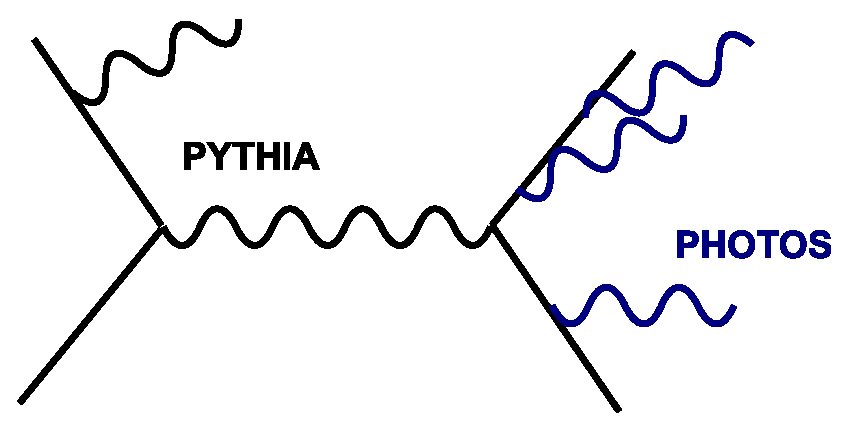
\includegraphics[width=0.9\textwidth]{figs/pyth-photos.eps}
  \end{columns}

  \vspace{0.3cm}
  В дополнение в {\color{red}SANC} реализованы следующие поправки {\color{red}NLO EW}:
  \begin{itemize}
    \item чисто слабые {\color{red}(PW)};
    \item интерференция между начальным и конечным QED излучением ({\color{red}IFI)};
    \item оставшиеся от ISR после вычитания {\color{red}коллинеарных расходимостей}.
  \end{itemize}
%  Данные поправки могут быть оценены {\color{blue!40!gray}вычитанием} FSR QED-компоненты  из
%  полных NLO EW поправок: SUPL=NLO-FSR.
}


\frame{
  \frametitle{Оценка дополнительные поправок}
  Дополнительные поправки зависят от кинематических ограничений: например, для
  процесса {\color{blue!40!gray}\(pp\to Z\to\mu^+\mu^-\)} поправки к распределению по
  \(M_{\mu^+\mu^-}\) меняются {\color{red}от \(-1\%\) до \(5\%\)} вокруг \(Z\)-резонанса,
  что делает необходимым их учёт в анализе
  \begin{align*}
  \delta_{\bar{X}}= \frac{\mathrm{d}\sigma_{\bar{X}}^{\mathrm{SUPL}}}{\mathrm{d}\sigma_{\bar{X}}^{\mathrm{LO}}},\quad \%
  \end{align*}
  \begin{columns}
  \column{0.5\textwidth}
  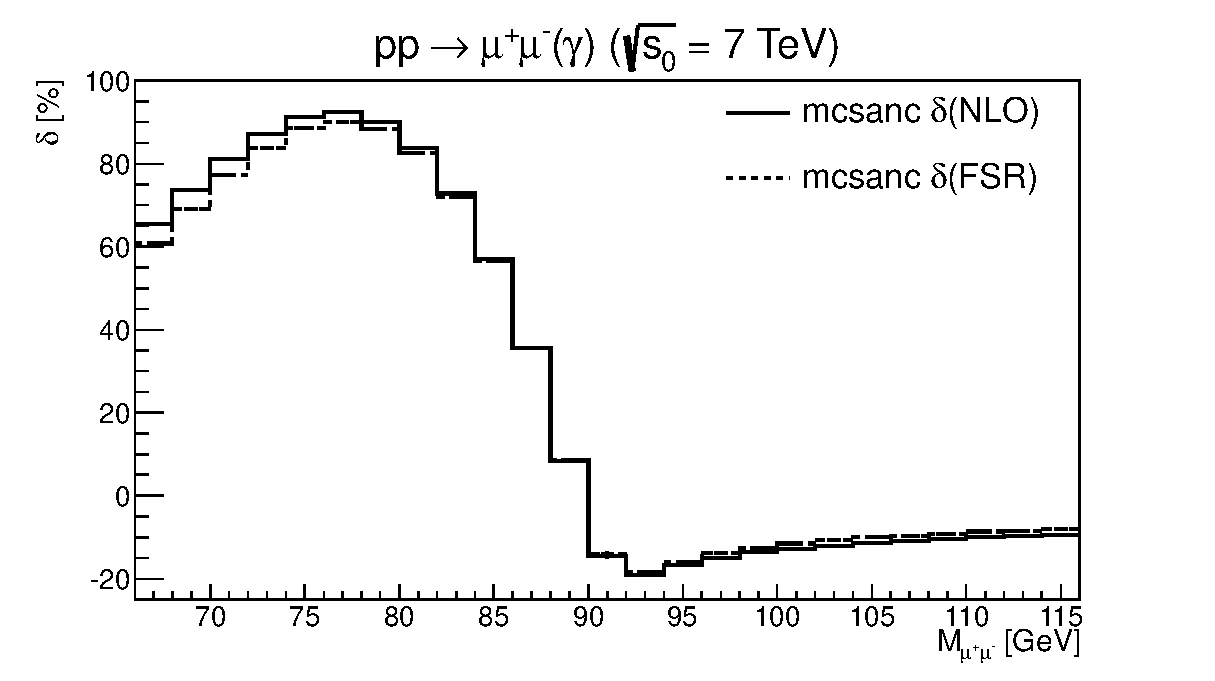
\includegraphics[width=1.1\textwidth,height=0.6\textwidth]{figs/miv_nlo_fsr_dlt.eps}
  \column{0.5\textwidth}
  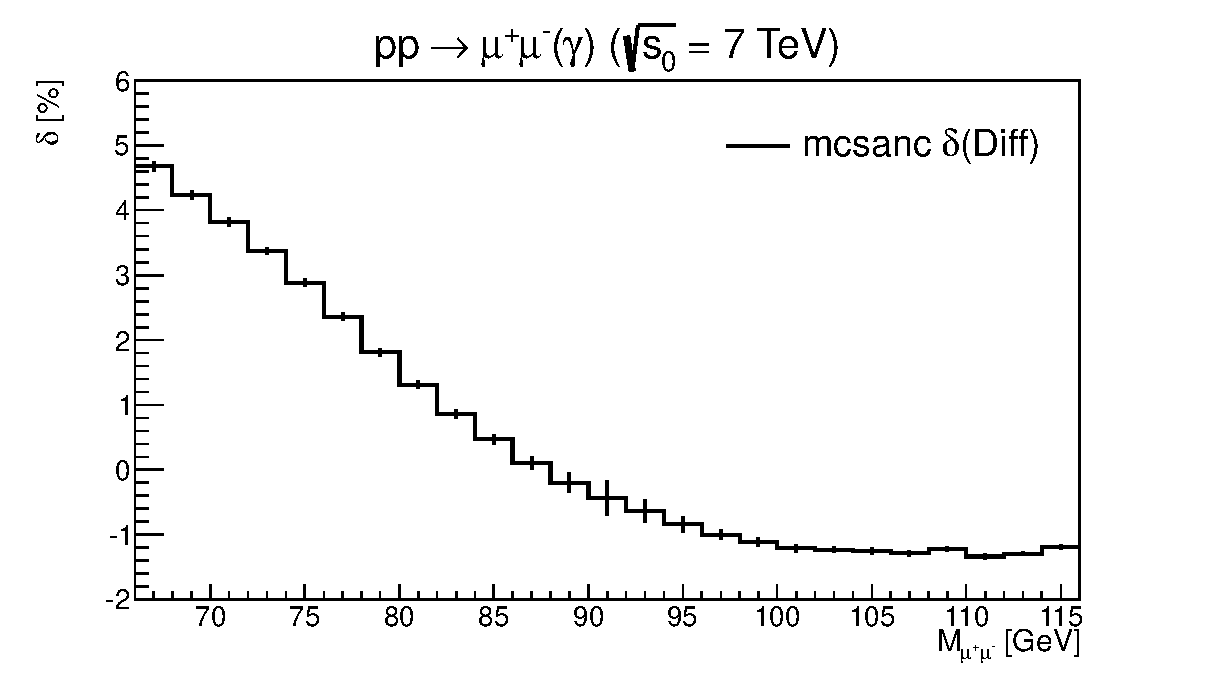
\includegraphics[width=1.1\textwidth,height=0.6\textwidth]{figs/miv_mispr_dlt.eps}
  \end{columns}
  \vspace{0.5cm}
}


\frame{
  \frametitle{Характеристики метода SANC}

  \begin{center}
  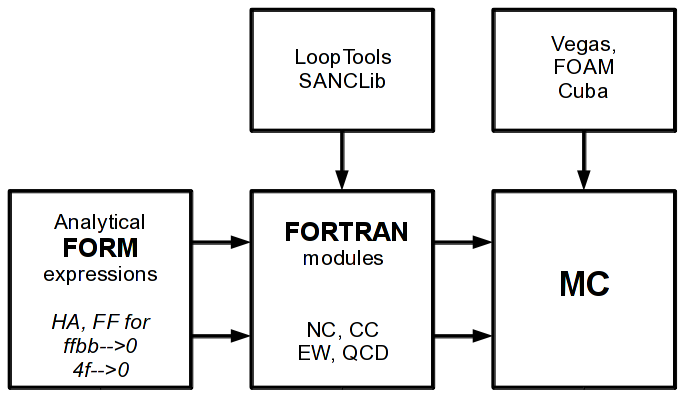
\includegraphics[width=0.6\textwidth,height=0.3\textwidth]{figs/sanc-scheme.png}
  \end{center}
  {\small
  \begin{itemize}
  \item Вычисления производятся в схеме перенормировки на массовой поверхности в \(R_{\xi}\) калибровке;
  \item Полное сечение NLO делится на несколько вкладов. Например, для электрослабых поправок: \\
  \vspace{-0.5cm}
\begin{align*}
\sigma^{\mathrm{NLO EW}} = \sigma^{\mathrm{Born}}
+\sigma^{\mathrm{virt}}(\lambda)
+\sigma^{\mathrm{soft}}(\lambda,\bar{\omega})
+\sigma^{\mathrm{hard}}(\bar{\omega})
+\sigma^{\mathrm{subt}}
\end{align*}
  \item Поддерживаются схемы вычитания \(\overline{\mathrm{MS}}\) и DIS.
  \item На основе модулей SANC было создано несколько Монте-Карло программ, в том числе интегратор \texttt{mcsanc}
  \end{itemize}
  }
}

\frame{
  \frametitle{Свойства интегратора \texttt{mcsanc}}
  \begin{itemize}
  \item Вычисляет {\color{blue!40!gray}полностью дифференциальное сечение} для ряда процессов 
        протон-протонных столкновений для условий LHC;
  \item Позволяет вычислять {\color{green!80!black}электрослабые и QCD NLO} поправки;
  \item Различные электрослабые схемы (\(\alpha(0), \alpha(M_Z), G_{\mu}\) ) и шкалы факторизации и перенормировки;
  \item {\color{blue!40!gray}Параллелизация вычислений} для многоядерных процессоров благодаря библиотеке Cuba (http://www.feynarts.de/cuba/)
  \end{itemize}

  {\small
  \begin{center}
  \begin{tabular}{|l|c|c|}
  \hline
  pid & \(ff\to\) \\
  \hline
  001:003 & \(l^+l^- (l=e,\mu,\tau)\)  \\
  004 & \(Z^0+H\)  \\
  \hline
  \(\pm\) 101:103 & \(l^{\pm} +\nu_l \)  \\
  \(\pm\) 104 & \(W^{\pm} +H \) \\
  \hline
  105 & \(t+\bar{b} \) (s-channel) \\
  106 & \(t+q \) (t-channel)  \\
  -105 & \(\bar{t}+b \) (s-channel) \\
  -106 & \(\bar{t}+q \) (t-channel) \\
  \end{tabular}
  \end{center}
  }
}


\frame{
  \frametitle{Сравнения с MCFM и FEWZ (EW)}
  Проводились для условий LHC при \(\sqrt{s_0} = 14\)TeV
  \begin{columns}
  \column{0.55\textwidth}
    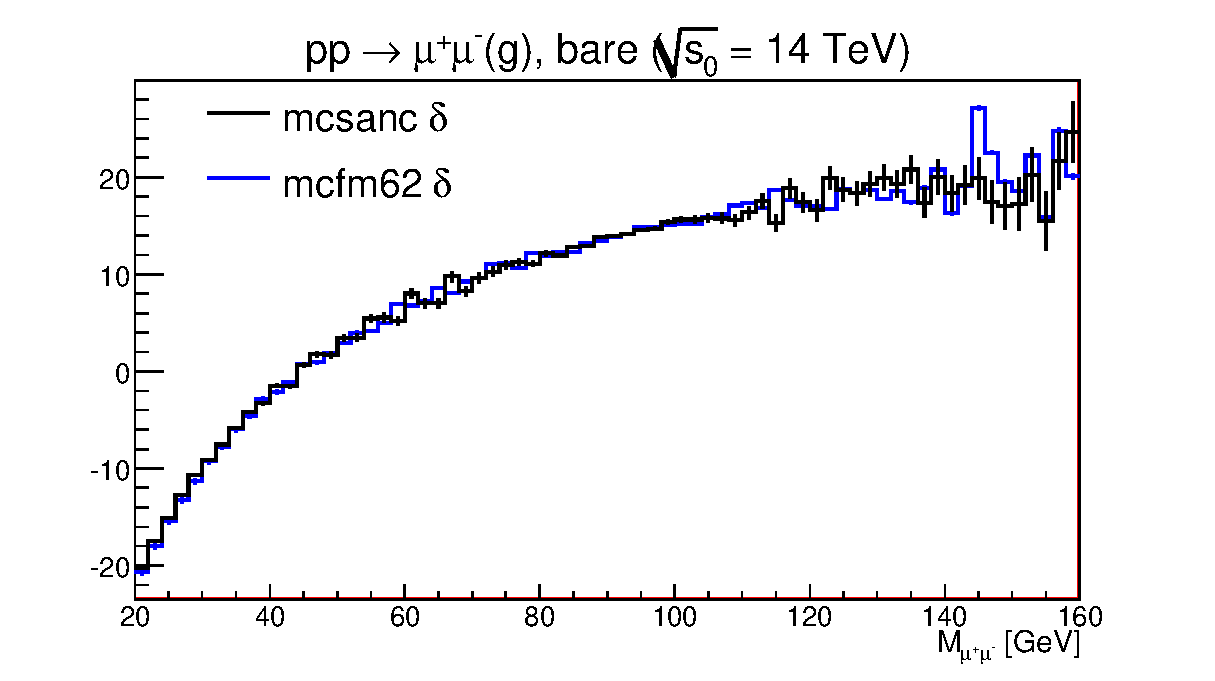
\includegraphics[width=0.98\textwidth]{figs/nc_dy_nlo_qcd_nocut_hist_mu_d34-bare_mcsanc_vs_mcfm62.eps}\\
    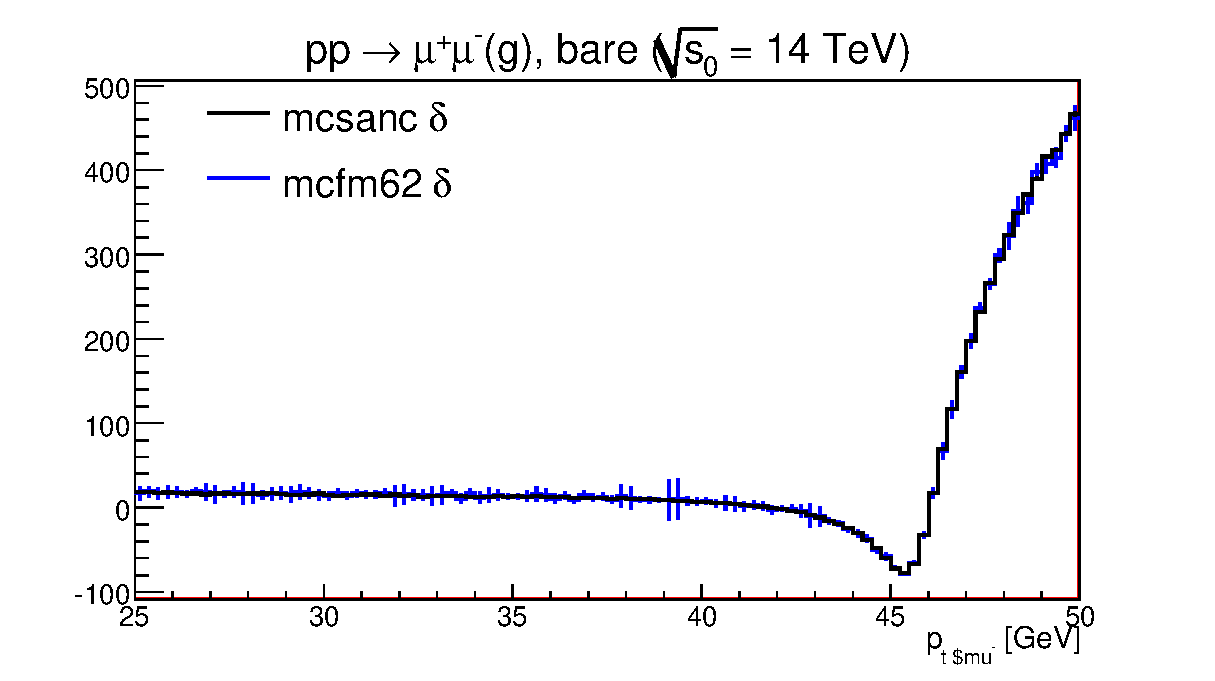
\includegraphics[width=0.98\textwidth]{figs/nc_dy_nlo_qcd_nocut_hist_mu_dt4-bare_mcsanc_vs_mcfm62.eps}
  \column{0.45\textwidth}
  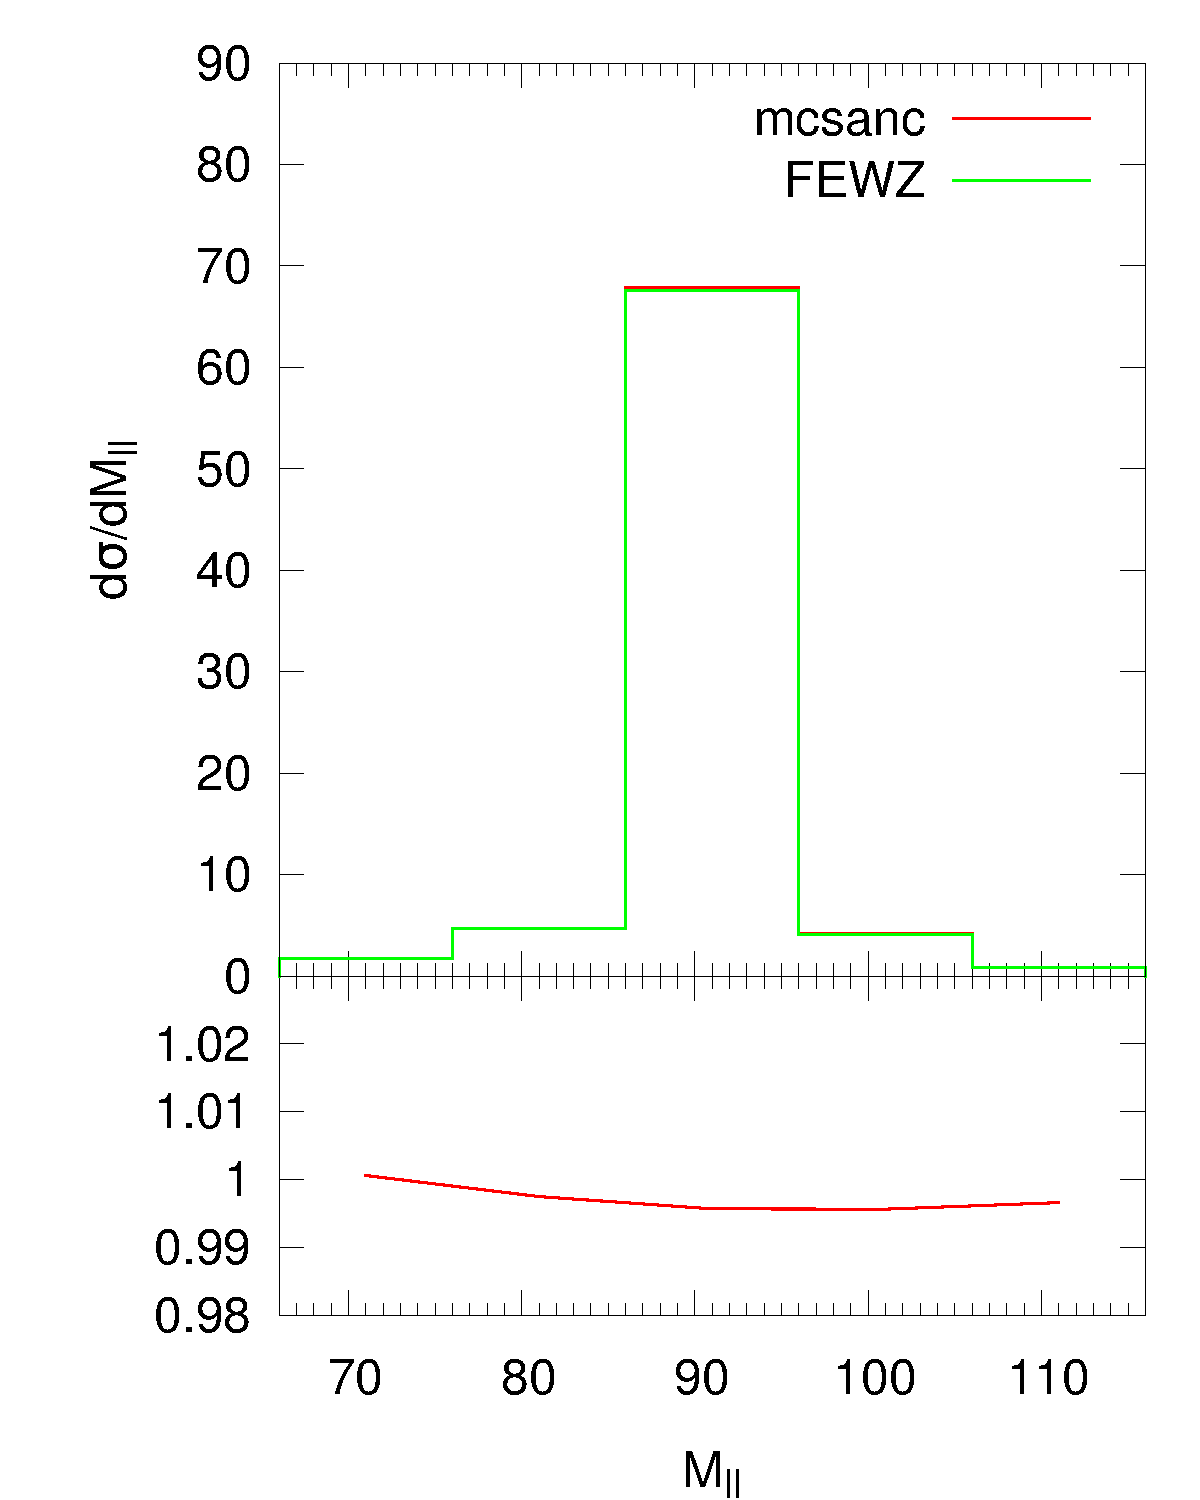
\includegraphics[width=\textwidth]{figs/dy-LObased.pdf}
  \end{columns}

}


\frame{
\vspace*{-2mm}
\frametitle{Дополнительные поправки для анализа ATLAS.} 

\vspace*{3mm}

\begin{minipage}{12cm}

  \begin{itemize}
  \item Производился на данных, набранных за 2010-2012гг, с интегральной светимостью более {\color{blue!40!gray}\(25\mathrm{fb}^{-1}\)}.
  \item Для анализа {\color{blue!40!gray}рождения W/Z бозонов} в SANC
    вычислялись электрослабые NLO поправки.
  \item Дополнительные поправки вычислялись для \(M_{\ell\ell}\) в диапазонах 
    {\color{blue!40!gray}\(26\text{--}66\), \(66\text{--}116\) и \(116\text{--}1500\)GeV}.
  \item Также вычисления электрослабых поправок SANC использовались при 
    QCD-анализе данных ATLAS за 2010г, в котором было измерено {\color{blue!80} соотношение
    плотности морских \(s\)- и \(d\)-кварков}.
  \end{itemize}
  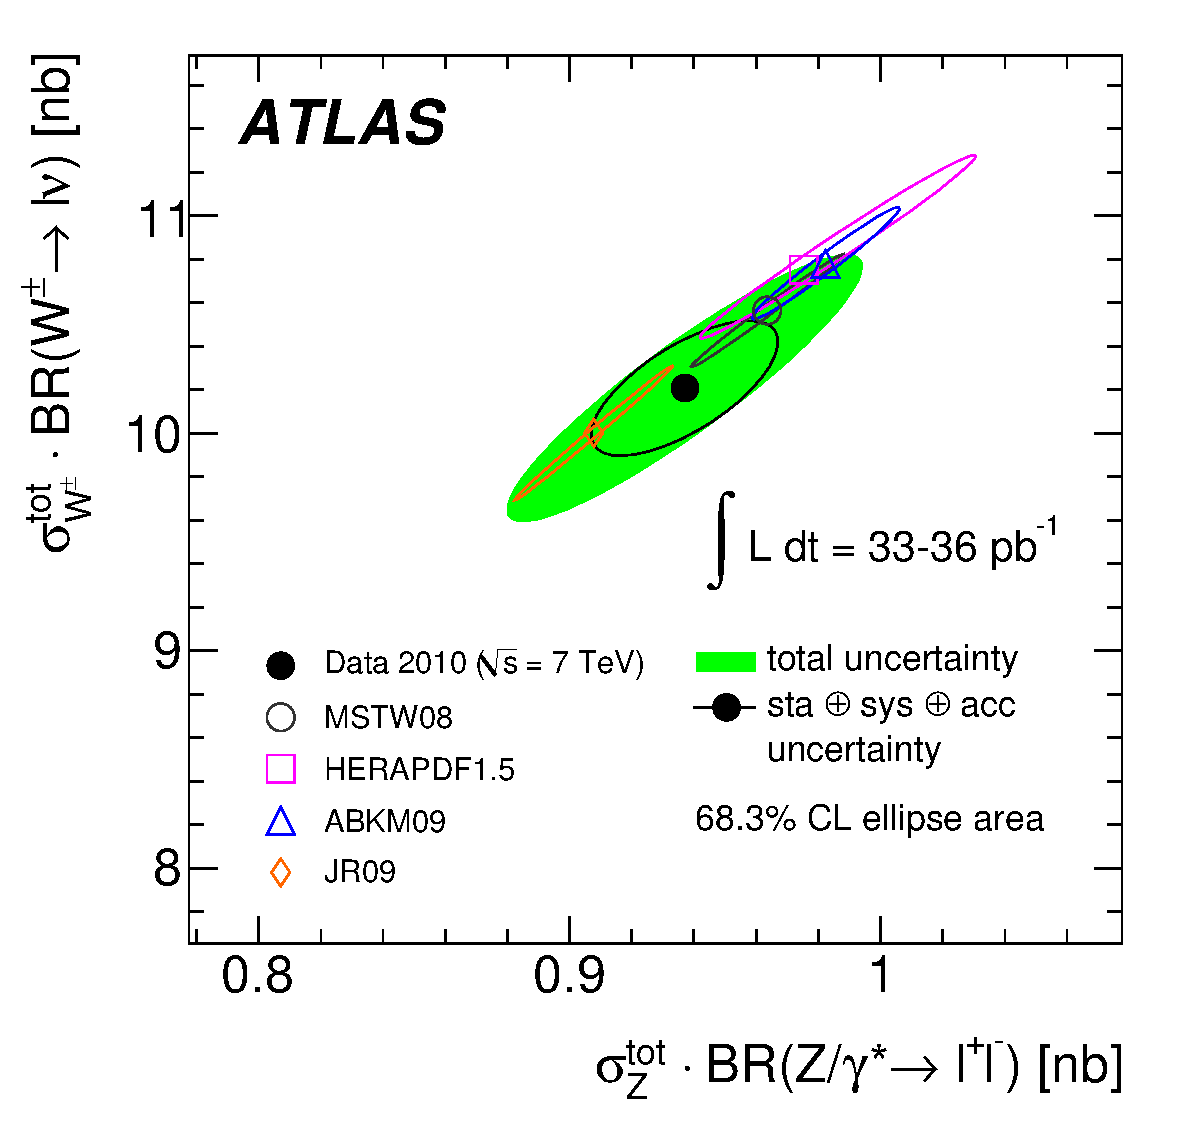
\includegraphics[width=0.3\textwidth]{figs/lepWZPlot_tot_tel-eps-converted-to.pdf}
\hspace*{2mm}
  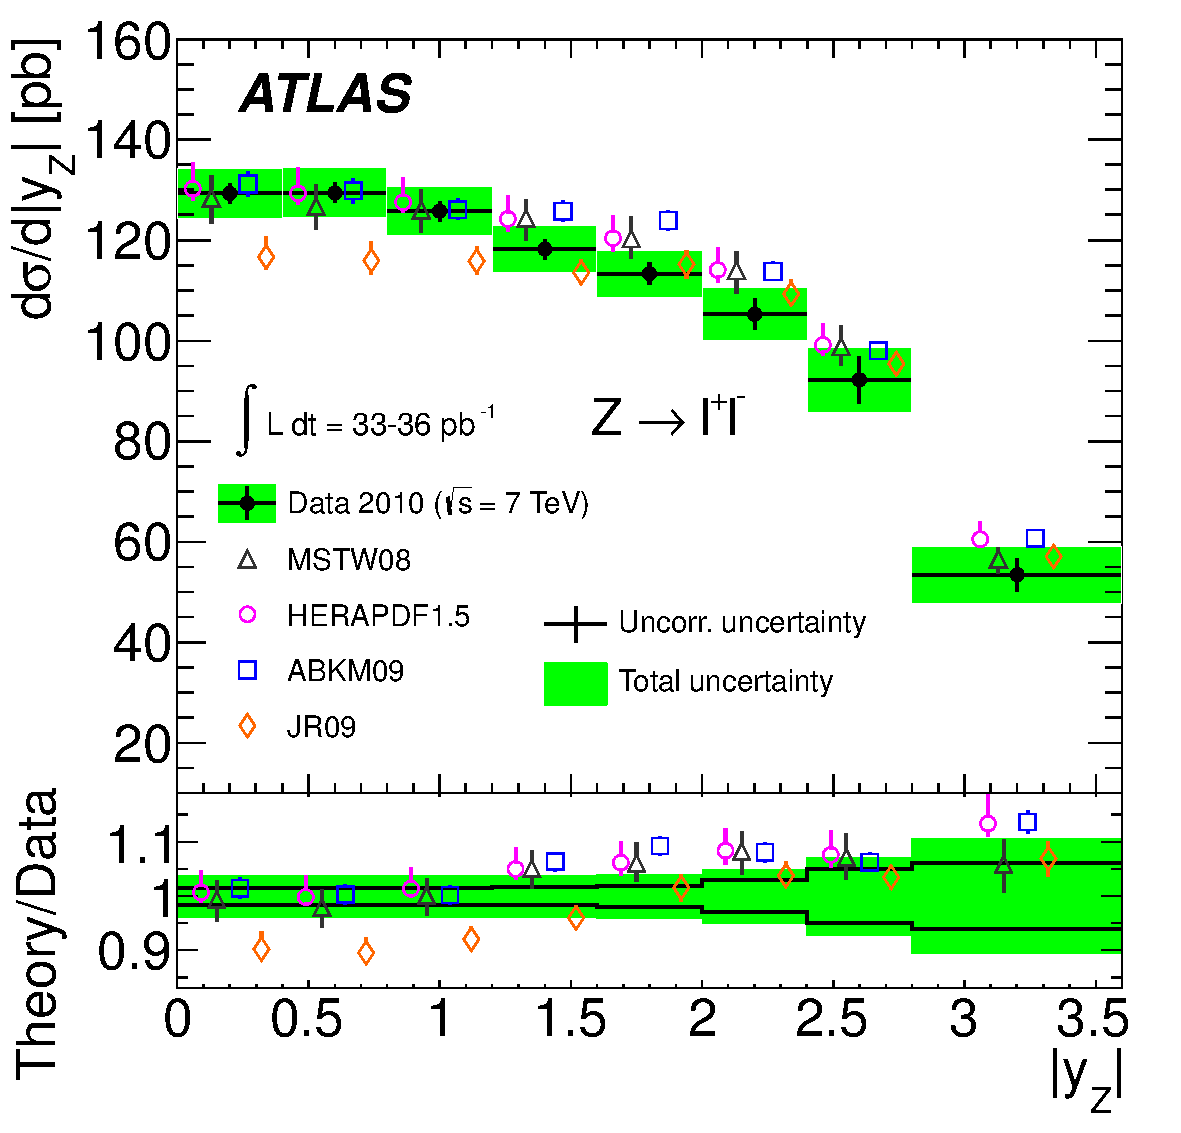
\includegraphics[width=0.3\textwidth]{figs/z_combined_theory_ratio-eps-converted-to.pdf}
\hspace*{2mm}
  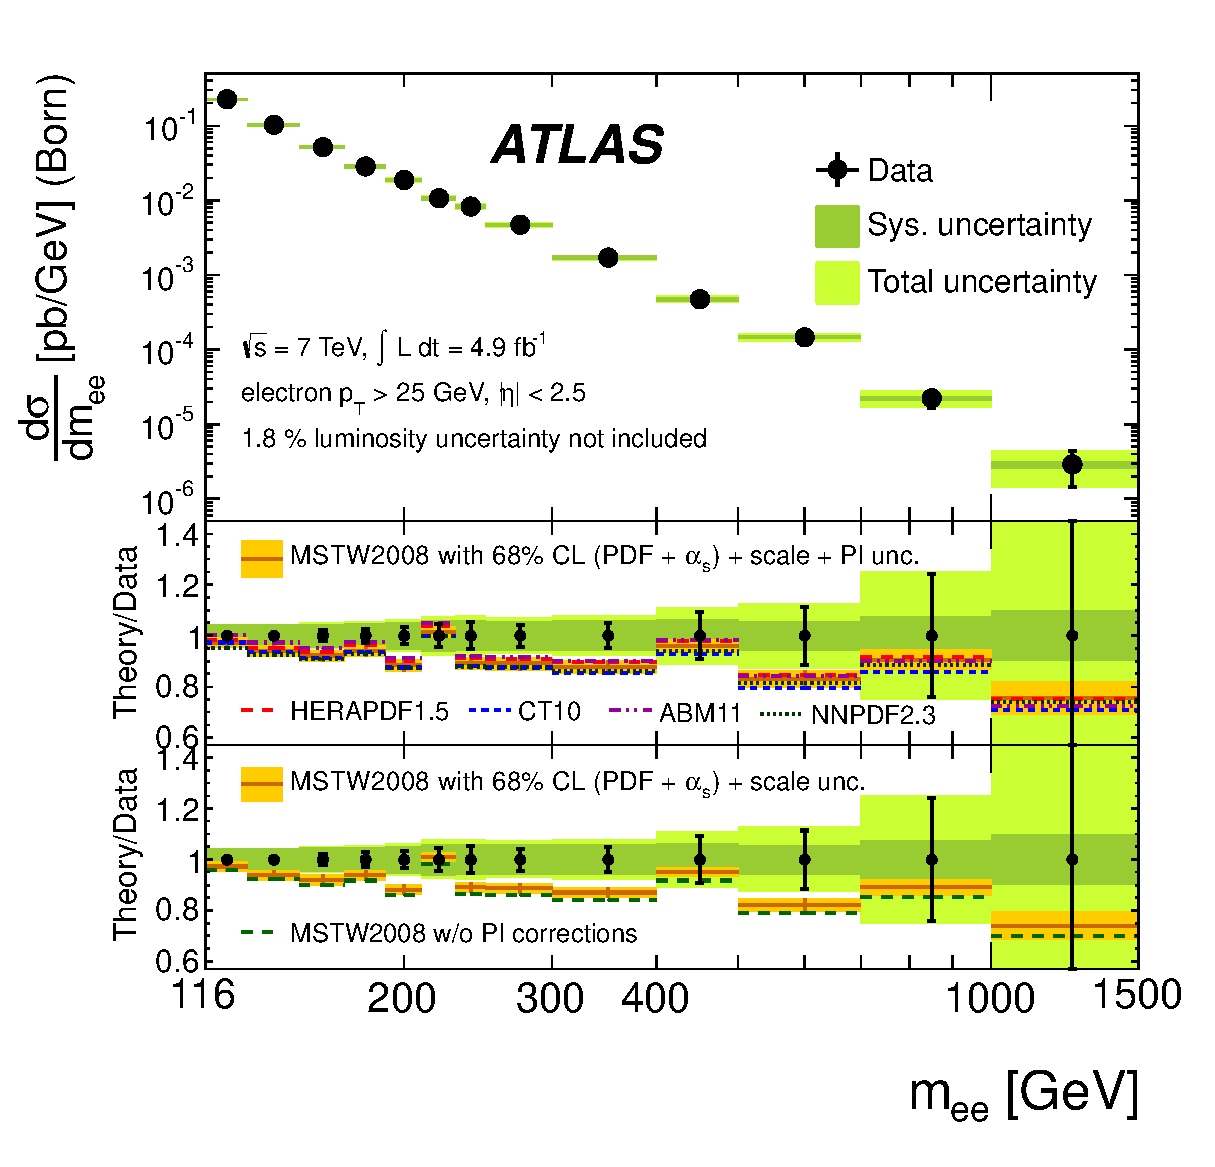
\includegraphics[width=0.3\textwidth]{figs/CS_fidcom_born_FEWZ_theoryData_withrealWZradiation_bothUnc.eps}
\end{minipage}
}

\frame{
  \frametitle{Заключение}
  \begin{itemize}
  \item Группа SANC разработала интегратор {\tt mcsanc}, вычисляющий {\color{red!80} одновременно
    NLO QCD и EW-поправки} к ряду процессов, включая процессы типа Дрелла--Яна.
  \item Программа {\color{blue!80} ориентирована на физику LHC} и позволяет получать дифференциальные
    распределения различных наблюдаемых при требуемых входных параметрах и
    кинематических ограничениях.
  \item {\color{green!80!black} {\tt mcsanc} активно используется для вычисления дополнительных 
    поправок, необходимых для проведения анализа процессов типа 
    Дрелла--Яна в эксперименте ATLAS.}
  \end{itemize}
}

\end{document}
